
In this chapter an example program will be introduced
which will be used to explain the use of the program analysis tools.
The basic routine of instrumentation, testing and analyzing will be discussed
to get acquainted with the tool set.


\section{Example Program}
\label{s:exampleProgram}

An example program called \verb|textVal| has been created to output some value based on an input text.
The value is calculated in the following way. 
For each letter of the alphabet the value is incremented by one,
for each digit the value is incremented by two
and for any other printable, non-space character the value is increased by ten.
This is according to the following equation.
\begin{center}
\begin{tabular}{rl}
$l =$ & number of letters  \\
$d =$ & number of digits \\
$o =$ & number of other characters \\
$v =$ & $ l + 2*d + 10*o $ \\
\end{tabular}
\end{center}

For demonstration purposes this program is deliberately created using three separate threads,
each scanning for a different sort of character and incrementing a shared value.
The complete source code is given in Listing \ref{l:textVal}.
Two bugs are introduced, which relate to mutual exclusion.
The critical section of this code is at the \verb|updateVal| function,
which adds the value of its argument to the shared value containing the result of the program.
The thread that is responsible for reading letters of the alphabet,
running the \verb|readLetters| function,
correctly locks the mutex.
However it is assumed that other threads do the same,
which is not always the case and which in practice results in hard to find bugs.
In this case, the thread that scans for digits (\verb|readDigits|) does not lock and unlock the mutex,
which results in a critical section that is not exclusively executed by one thread at a time.
If the first thread reads the shared value at line 16 and 
the second thread reads the same value before the first thread has written a value back,
then information is lost and the resulting value will be lower than expected.

The second introduced bug in this code is located in the code of the third thread,
which scans for special characters
using the function \verb|readOthers|.
This thread does lock the mutex, but does not release the exclusive right to the critical section,
resulting in a situation in which the first thread waits forever for the mutex to become unlocked.

\lstinputlisting
	[label=l:textVal, caption=source code for the textVal example program]
	{sources/textVal.c}

In the next sections an example analysis is made for the \verb|textVal| program.
In order to analyze the program we first have to instrument the code to 
have it keep a record of executed portions of code (a program spectrum).
This instrumented program is then run with different test inputs,
some resulting in correct output values, others failing to produce the correct value.
The data that is gathered during these tests is analyzed and 
this results in a list of possible locations of the fault.

	
\section{Instrumentation}
\label{s:instrumentation}
	
	First, the program has to be instrumented to create execution data during the tests.
	When running the instrumented program, 
	a counter corresponding to an instrumented piece of code is incremented 
	each time that piece of code is executed.
	This results in a spectrum of the execution of the program.
	
	Different types of program points can be instrumented.
	The tool set supports, for example, function level instrumentation
	and instrumentation at the basic block level, 
	but also supports custom instrumentations.
	Detailed information of instrumenting program points for creating
	program spectra is given in Chapter \ref{c:ProgramSpectrumGeneration}.
	
	Instrumentation is done by the \verb|instrument| tool.
	In our case we will instrument each basic block of the program.
	A basic block is defined as a sequence of statements with one entry point and one exit point,
	having no jump instructions contained within it.
	The following commands are used to instrument the program.\\
	\verb|  # llvm-gcc -g -emit-llvm -c textVal.c -o textVal.bc| \\
	\verb|  # instrument -f -spbasicblock -bypassmain -memprotection \ | \\
	\verb|  > textVal.bc -o textVal.ibc| \\
	\verb|  # llc -f textVal.ibc -o textVal.s| \\
	\verb|  # gcc textVal.s -lpthread -linstrument -o textVal| \\
	
	The first line uses the \verb|llvm-gcc| compiler to create \verb|llvm| \emph{intermediate byte code}.
	Care must be taken to include the \verb|-g| option to generate debug information,
	which is required during instrumentation.
	The \verb|-emit-llvm| and \verb|-c| options result in the creation of the byte code, 
	in stead of trying to create an executable.
	
	The second line is the actual instrumentation.
	The \verb|instrument| tool accepts multiple \emph{instrumentation passes},
	the \verb|-spbasicblock| pass being one of them.
	The \verb|-spbasicblock| option adds instrumentation of basic blocks.
	The \verb|-memprotection| option guarantees that the instrumented program
	will not be able to accidentally invalidate the data that is gathered during run-time.
	In order to achieve this, every store operation is checked to ensure it will not
	modify the part of memory which contains the instrumentation data.
	The \verb|-bypassmain| option bypasses the main function of the program,
	in order to initiate instrumentation data and to handle exceptions while
	not losing recorded data.
	Finally, the \verb|-f| option forces to overwrite existing output data.
	The output is an instrumented form of the \verb|llvm| byte code.
	
	The third line contains another \verb|llvm| tool to create native code from the 
	\verb|llvm| byte code.
	Again, the \verb|-f| option ensures that an existing output file is overwritten
	without complaining.
	
	The final line uses \verb|gcc| to link the resulting native code with 
	the \verb|pthread| library and with the \verb|instrument| library.
	The latter contains the functionality for initializing spectrum data,
	starting the instrumented program, handling spectrum updates and
	writing results into a datafile.
	
	At this point we have an executable program,
	which behaves as the original program would behave,
	with the added functionality of creating a program spectrum.
	In the next section we will create some test cases and 
	perform an analysis to locate the faults.
	

\section{Testing}

	In most software projects, tests are created along with the software itself.
	During the implementation and testing phases these tests are used to validate
	the functionality of the software.
	Failing tests indicate which features of the software are incomplete or faulty.
	However, software bugs are often not directly traceable to lines of code.
	Even test-driven implementation using unit tests will in many cases prove insufficient 
	to build bug free code.
	A piece of code can contain a fault which did cause an error in small tests
	but will lead to a failure when integrated into a larger code base.
	
	For the example program, a number of tests were created. 
	These include testing only letters for input, 
	only digits or special characters, or combinations of character types.
	These are standard tests to verify the functionality of the program.
	A problem in this case is that some small tests will work as expected,
	but will fail if they are scaled up.
	The mutex problem is the cause of this irregular behavior, 
	since task switching between the threads will unlikely occur 
	during the scanning of small input.
	
	\begin{table}
		\begin{center}
		\begin{tabular}{l|l|r r r|r|r}
			\hline
			          &       & \multicolumn{3}{c|}{summary} & expected & textVal \\
			test file & input & $l$ & $d$ & $o$ & output & output \\
			\hline
			test1.in & \verb|"abcdefghij"|   & $10$   & $0$   & $0$ & $10$   & $10$ \\
			test2.in & \verb|"0123456789"|   & $0$    & $10$  & $0$ & $20$   & $20$ \\
			test3.in & \verb|"A0B1C2D3E4"|   & $5$    & $5$   & $0$ & $15$   & $15$ \\
			test4.in & large text only       & $1040$ & $0$   & $0$ & $1040$ & $1040$ \\
			test5.in & large text and digits & $520$  & $200$ & $0$ & $920$  & $< 920$ \\
			test6.in & \verb|".=+-#"|        & $0$    & $0$   & $5$ & $50$   & hangs \\
		\end{tabular}
		\end{center}
		\caption{Test suite for the textVal program with information on the number of 
		letters, digits and other characters.}
		\label{t:TestSuite}
	\end{table}
	
	Table \ref{t:TestSuite} shows the test suite that is available for this program.
	The input, or a description of the input, is given 
	together with a summary in terms of the number of letters, digits and other characters.
	For each test also the expected output is given and the actual output of the program.
	
	First, test 1 to 5 are run, since test 6 shows different behavior than the incorrect output.
	These tests are run as follows.\\
	\verb|  # ./textVal < test1.in|\\
	\verb|  # ./textVal < test2.in|\\
	\verb|  # ./textVal < test3.in|\\
	\verb|  # ./textVal < test4.in|\\
	\verb|  # ./textVal < test5.in|\\
	You will see the correct output for the first four tests.
	Most likely, test 5 yields a value which is less than the expected value of 920.
	Test 6 results in the hanging of the program and will be discussed
	in Chapter \ref{c:AutomaticErrorDetection} (it should not yet be executed at this point).
	Note that, in practice, we have no real clue what the cause would be.
	We see that a text with mixed letters and digits works as expected,
	given that the size of the text is limited, but the same test fails if the text size is large.
	In conventional debugging one could be mislead by these results and would start looking at
	the text buffer or the reading of the input.
	In this case we use a black box method.
	A program is instrumented and run in the same way the original program would have been run.
	
	
\section{Analysis}

	The resulting run data of the test runs is stored in a separate file called \verb|datafile.dat|.
	This file is created after the first run and is incrementally updated at every next run.
	This data file contains program spectrum information, among other things.
	Before we can start the analysis using the \verb|zoltar| tool,
	first we need to specify which test runs have failed and which have passed.
	This can be done in two ways.
	The pass and fail information can be stored in a separate file, 
	containing a '1' for each passed test and a '0' for each failed test.
	This is very useful for running a batch of tests and is explained in Chapter \ref{c:BatchExecution}.
	The second method is through the \verb|zoltar| tool itself, 
	which is what will be shown next.
	
	The \verb|zoltar| tool can be started by typing\\
	\verb|  # zoltar|\\
	in the directory where the tests have been run.
	The \verb|datafile.dat| file is then automatically opened.
	The same holds for a context file called \verb|context.dat|.
	If the program has been instrumented in another directory the
	\verb|context.dat| file will be located in that directory.
	It contains the source file location for each instrumented program point
	to enable the mapping of probable fault locations in the executable 
	to the pieces of code in the original source file.
	In case the context file is located elsewhere, 
	the location can be passed with the following option.\\
	\verb|  # zoltar --contextfile=/path/to/context.dat|\\
	It might be wise to look at more options using the command:\\
	\verb|  # zoltar --help|\\
	Most options will be discussed in the remainder of this tutorial.
	
	When the tool is started the main menu is shown and is active.
	In the right hand window a summary of the instrumented program and the test runs is given,
	like the number of runs and the number of spectra that were instrumented.
	Changing the pass and fail information of the runs is done in the \verb|runs| submenu.
	This can be selected by pressing \emph{down} on the keyboard to navigate to the \verb|runs|
	entry in the main menu and by pressing \emph{enter}.
	The test runs are then listed and each run can be selected to change its status to \emph{passed}
	or \emph{failed}.
	In our case we will change the fifth run to \emph{failed}, 
	since the output of this run was not what we expected it to be.
	Figure \ref{fig:analyzeRuns} shows the screen of the \verb|zoltar| tool at this point.
	
	\begin{figure}[h!]
		\begin{center}
		\begin{tabular}{c}
			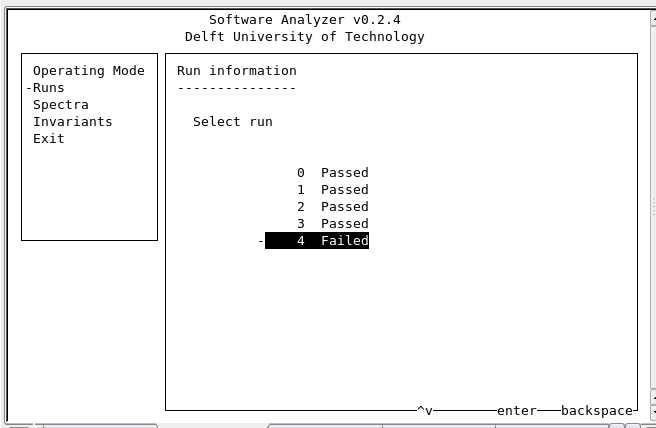
\includegraphics[scale=0.40]{sources/analyze_runs.png} \\
		\end{tabular}
		\end{center}
		\caption{The test run information of the textVal tests.}
		\label{fig:analyzeRuns}
	\end{figure}

	\begin{figure}[h!]
		\begin{center}
		\begin{tabular}{c}
			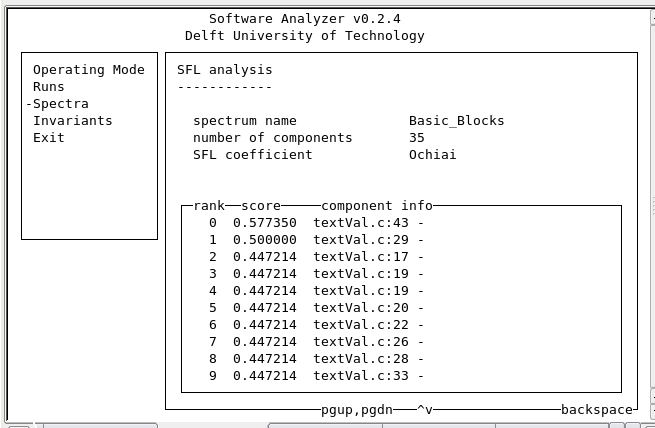
\includegraphics[scale=0.40]{sources/analyze_sfl.png} \\
		\end{tabular}
		\end{center}
		\caption{SFL results of the textVal tests.}
		\label{fig:analyzeSfl}
	\end{figure}
	
	The keys that can be used in each screen are shown at the bottom of the screen.
	To go back to the previous screen the '\emph{backspace}' key can be pressed.
	Back in the main menu the \verb|Spectra| entry can be chosen to investigate the
	program spectrum of the basic blocks, which we have created during the test runs.
	To do this, select the \verb|Spectra| entry, then select \verb|Basic Blocks| 
	in the \verb|select spectrum| screen.
	At this point we can choose to inspect the spectrum data 
	or perform SFL on the data.
	We will select the \verb|Perform SFL analysis| option and select the
	\verb|Ochiai| similarity coefficient.
	Other coefficients are also possible, but are present for research purposes.
	The \verb|Ochiai| coefficient is known to be the best performing coefficient.
	
	Spectrum-based fault localization (SFL) returns a list of program locations
	sorted by the probability of the fault being at that location.
	The location can be a basic block, a function or another unit of code,
	depending on the instrumentation that is performed.
	The probability is calculated by looking at the correlation of the execution of each instrumented
	program point with the failing of test runs.
	If some points of the program get to be executed whenever the program fails to produce the
	expected output, then these points are good candidates for inspection.
	
	In our case, sometimes the piece of code containing the bug is executed without causing
	faulty behavior.
	This is, unfortunately, the case in many situations.
	In general, having more test cases also gives more information of the correlation of certain locations and
	failing runs.
	Nevertheless, SFL will rank that code high, as explained in Chapter \ref{c:SFL}.
	Figure \ref{fig:analyzeSfl} shows the ranked list which is the output of the \verb|zoltar| tool.
	It shows that line 43 in the \verb|textVal.c| source file ranks highest 
	and therefor is the most probable location containing a bug.
	
	To quit the program you can press the '\emph{backspace}' key until the main menu is active,
	after which \verb|exit| can be selected.
	Alternatively, the '\emph{q}' key can be pressed at any time to quit.
	
	For a better visualization of this ranking in the source code
	a graphical analysis tool is available as well.
	This \verb|xzoltar| tool can be started in the same way as the \verb|zoltar| tool,
	specifying the context and data files in the same way using the same options.
	Typing \\
	\verb|  # xzoltar|\\
	or, if the context file is located elsewhere,\\
	\verb|  # xzoltar --contextfile=/path/to/context.dat|\\
	on the command line will show a graphical representation of the same ranked list as
	presented in the \verb|zoltar| tool.
	Each instrumented block of code is color coded, 
	where red specifies a large SFL score and thus will be more
	likely to be the location of the fault.
	A green line will have little correlation with the failure.
	Actually, only the first line of the instrumented block of code is colored.
	Note also that LLVM can generate additional basic blocks
	(e.g. a \verb|}| at the end of a function could be considered an
	implicit return statement by LLVM).
	Next to this \emph{ranked list} tab there are tabs for each instrumented source file.
	In these files the lines which are present in the ranking have the same coloring.
	This makes it easy to locate areas of interest in each file and to 
	view the surrounding code and have some context of why the specified location would
	possibly be at fault.
	
	\begin{figure}[h!]
		\begin{center}
		\begin{tabular}{c}
			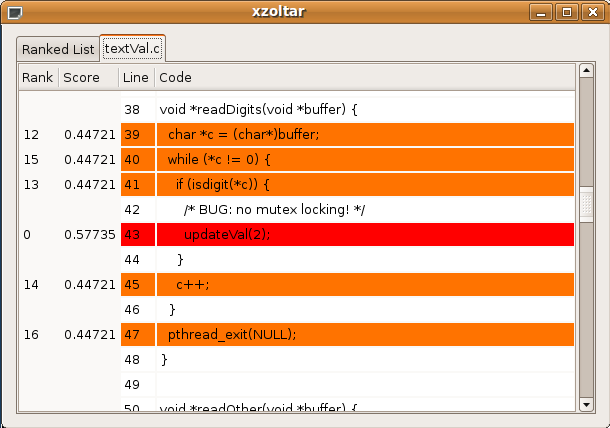
\includegraphics[scale=0.40]{sources/ganalyze_textVal.png} \\
		\end{tabular}
		\end{center}
		\caption{Visualization of SFL in the textVal source code.}
		\label{fig:ganalyzeTextVal}
	\end{figure}
	
	In Figure \ref{fig:ganalyzeTextVal} the \verb|xzoltar| tool shows the 
	highest ranking location in the code.
	It turns out that the call to \verb|updateVal| without locking the mutex
	correlates most with the failing test runs.
	Even without having been part of the implementation process,
	a person debugging this program could use this tool, get these results,
	and notice that another thread function does lock the mutex when calling the same function.
		
	It is important to realize that this tool will not explain why an error occurred.
	It statistically determines the most probable location a fault could reside.
	However, it gives a very useful starting point for inspecting the code.
	It can serve as a director in the debugging process,
	offering a list of source code locations to inspect.

	In some situations the gathered run-data becomes outdated.
	This happens when the test set is revised and a new test suite needs to
	be run starting with a clean sheet.
	Another possibility for outdated run-data is when the program
	is instrumented anew.
	This will invalidate the information in \verb|datafile.dat|.
	In these cases the datafile needs to be renamed or removed.
	After removal, the datafile is created again with the next test run.
	The instrumented program is able to detect if an existing datafile
	conflicts with the current instrumentation
	and will abort and give a message to that extend.
	Renaming the datafile could be used to save run-data for different
	test suites.
	The results of each suite can be examined at a later moment by 
	specifying the datafile as an argument to \verb|zoltar| (or \verb|xzoltar|):\\
	\verb|  # zoltar --datafile=/path/to/datafile.dat|\\

	This concludes the basic program analysis example.
	The next chapter will discuss the instrumentation for program spectra in more detail.
	Chapter \ref{c:AutomaticErrorDetection} will explain instrumentation of the program
	to enable automatic error detection.
	This is used to pinpoint the location for the second bug in the \verb|textVal| program.

	
	







% To analyze a program, its source code must be available.
% The program \emph{P} will be instrumented according to the needs and situation and will be transformed to \emph{P'}.
% Using the software package it is done in the following way.

% \begin{itemize}
  % \item{intermediate bytecode is generated\\
    % \verb| llvm-gcc -g -c program.c -o program.bc|}
  % \item{instrumentation is performed\\
    % \verb| instrument -spblock -memprotection -bypassmain program.bc > program.bc.p|}
  % \item{compile into native machine code\\
    % \verb| llvm-llc program.bc.p > program.s|}
  % \item{link with library and generate executable\\
    % \verb| gcc -linstrument program.s -o program|}
% \end{itemize}


	% Several optional instrumentation \emph{passes} are available.
	% These instrumentations can be categorized as follows.

	% \begin{itemize}
	  % \item{bypassing the main function}
	  % \item{instrumentation to generate program spectra}
	  % \item{instrumentation for program invariants}
	  % \item{memory protection}
	% \end{itemize}

	% There are some requirements for the input of the instrumentation.
	% \begin{itemize}
	  % \item{programs that are to be instrumented must contain a main function}
	  % \item{before instrumenting a program has to be pre-compiled to LLVM byte code}
	  % \item{pre-compilation should involve adding debug information (-g option)}
	% \end{itemize}

	% An important instrumentation pass, one that needs to be executed always,
	% is the pass that bypasses the \verb|main|